\subsection{実験概要}
提案手法によるより自然な敵対的サンプルが生成可能なのかどうか有効性を検証するため,敵対的サンプルの生成実験を行った.前述の通り,提案手法に示した重要度算出法と離散化手法を組み合わせ,敵対的サンプルを生成する.さらに,得られた敵対的サンプルの具体的な値について,適切か否かの確認を行う.
\subsection{実験条件}
今回の実験は,銀行のローンの審査システムについての機械学習モデルを想定し,誤分類を引き起こす敵対的サンプルの生成を行うことを目的とした.パラメータの設定は従来研究\cite{ballet2019imperceptible}に準拠している.今回使用する機械学習モデルは,12個の特徴量を入力とし,2つのクラス(承認または拒否)を出力するニューラルネットワークである.このネットワークは,100個のノードを持つ隠れ層が6層にわたって配置された全結合型のモデルである.隠れ層はReLU関数で活性化され,出力層はバイナリクラス分類のためにSoftmax関数が使用されている.これらのモデルを図示したものを下に示す.

\begin{figure}[H]
    \centering
    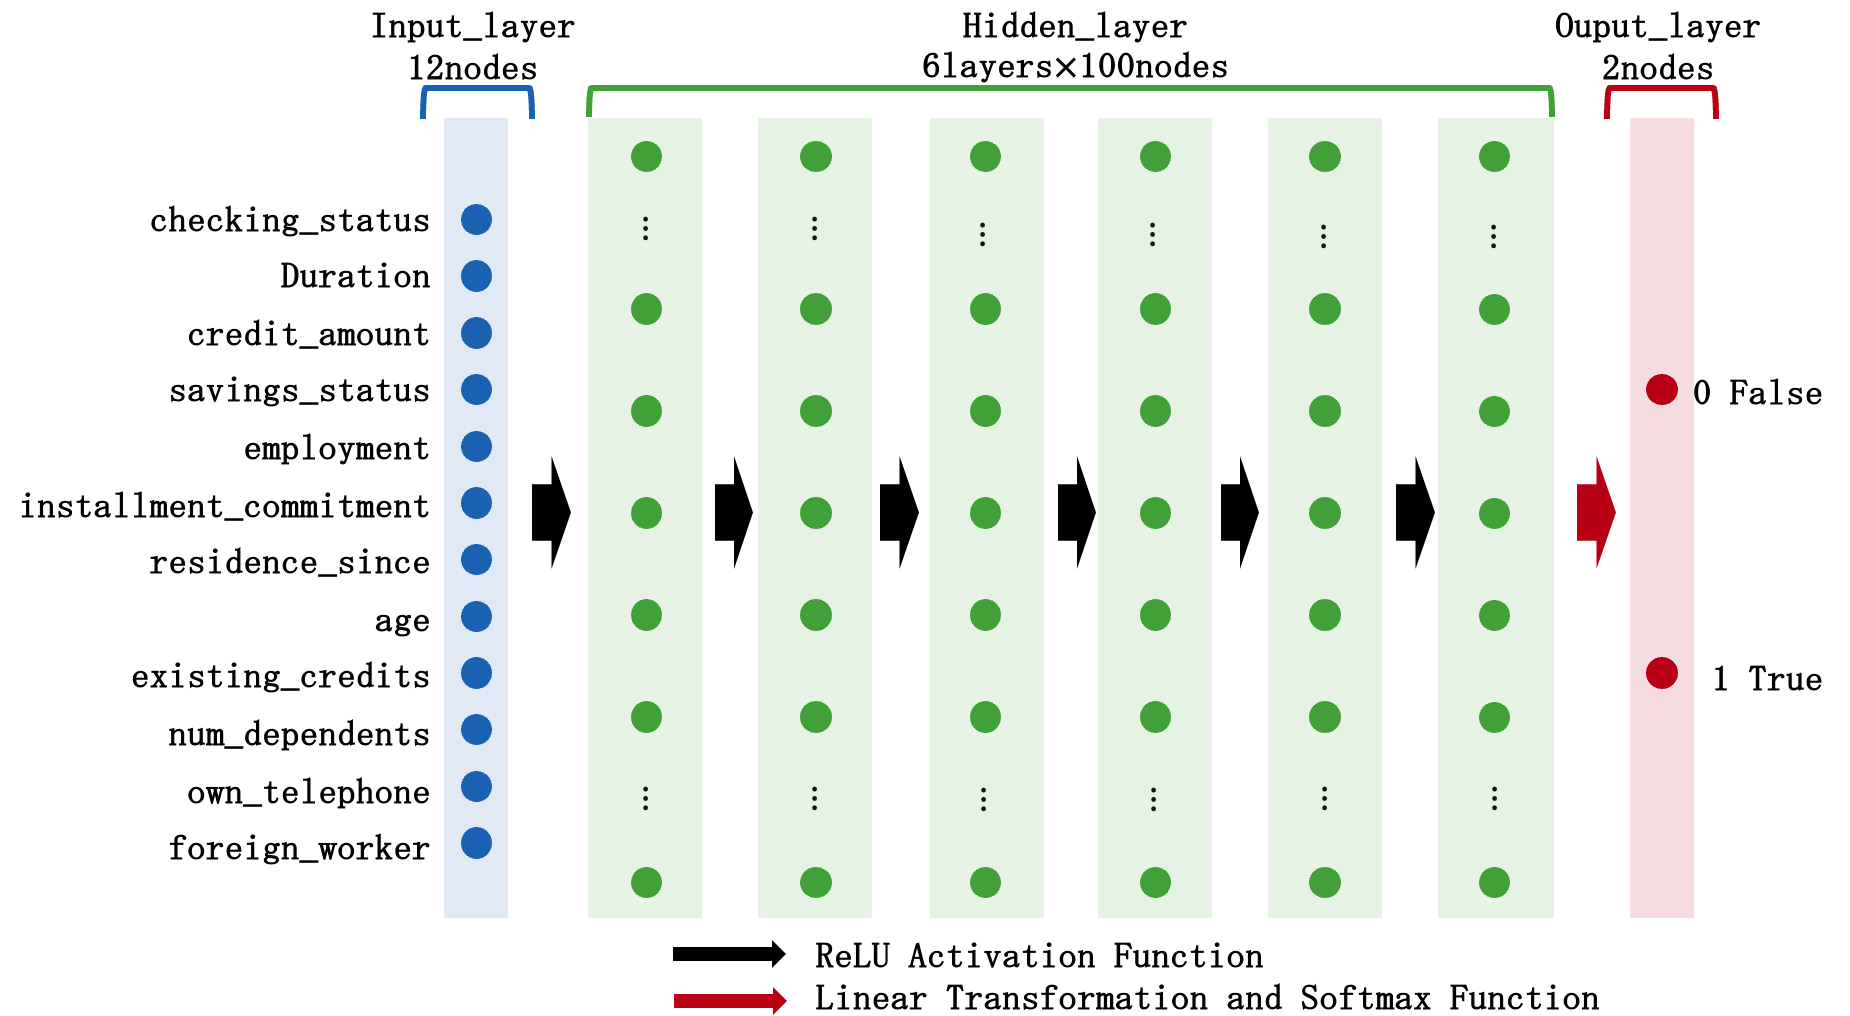
\includegraphics[width=0.8\textwidth]{images/審査モデル.png}
    \caption{銀行のローン審査を行う機械学習モデルの構造}
    \label{fig:adversarial_example}
\end{figure}

また,学習においてBCELoss(Binary Cross Entropy Loss)が損失関数として使用されている.モデルが各サンプルに対して予測した確率と実際のラベルとの誤差を計算し,二値分類における誤差を最小化する.最適化アルゴリズムにはAdamを使用し,学習率は $1.0 \times 10^{-4}$ に設定されている.バッチ学習を行い,バッチサイズは $N=100$ です.データを小分けにして学習を進め,予測精度はkeras.utils.to\_categoricalを用いてワンホットエンコーディングに変換し,各バッチで予測精度を計算した後,全データで平均を取っている.これによりモデルの分類精度を評価する.

使用データは前述のUCI Machine Learning RepositoryのGerman Credit Data Setを使用する.1000件のデータに対して正解データのバランスを保つようにデータをサンプリングする.取得した600件のデータのうち300件を学習データ,250件をテストデータ,残りを検証データに分割する.
まず,学習データでモデルの学習を行い,その後テストデータによるモデルの評価を行う.次にテストデータからランダムに10件取得し,それらをベースにノイズを加え敵対的サンプルを生成する.生成された敵対的サンプルに対して以下の評価指標を用いて評価を行う.

\subsection{評価指標}
提案手法の有効性の評価として以下の3つの指標を用い比較を行う.
一つ目に敵対的サンプルが元データと異なるクラスに分類されることを評価する指標である.これを成功率と呼び,式(9)に示す.
\autoequation{成功率 = \cfrac{|\hat{\mathbb{X}}|}{|\mathbb{X}|}}
ここで $\hat{\mathbb{X}}$ は生成された敵対的サンプルが元データと異なるクラスに分類されたサンプルの集合であり,$\mathbb{X}$ は全サンプルの集合である.この指標が大きいほど敵対的サンプルが元データと異なるクラスに分類されることが多いことを示す.

二つ目に敵対的サンプル生成前のサンプルと生成後のサンプル間の距離を評価する指標である.これを平均距離と呼び,式(10)に示す.
\autoequation{平均距離 = \cfrac{1}{N} \sum^{N}_{i=1} \sqrt{\sum^{d}_{j=1}(\mathrm{orig}_{i, j}-\mathrm{adv}_{i, j})^2}}
この指標が小さいほどノイズが小さく,元データに近いサンプルが生成されていることを示す.

三つ目に先ほどの平均距離に対して各特徴量の重要度で重み付けした指標である.これを重み距離と呼び,式(11)に示す.
\autoequation{重み距離 =  \cfrac{1}{N} \sum^{N}_{i=1} \sqrt{\sum^{d}_{j=1}( | \mathrm{orig}_{i, j}-\mathrm{adv}_{i, j}| \cdot v_i )^2}}
ここで使用する重要度 $\bm{v}$ は,従来手法で使用していた特徴量重要度 $\bm{v}$ と同様のものを使用する.この指標が小さいほど分類に対する重要度の高い特徴量に対するノイズが小さいことを示す.

各指標を組み合わせて使用することで,生成した敵対的サンプルの「有効性」と「自然さ」の両面を総合的に評価することを目指す.

\subsection{実験結果}
まず成功率について確認する.
\begin{table}[H]
    \centering
    \caption{実験結果:成功率}
    \begin{tabular}{|c|c|c|c|} \hline
        離散化 & 従来手法(式(6)) & 重要度算出(式(7)) & 重要度算出(式(8)) \\ \hline
        なし & 1.0 & 1.0 & 1.0 \\ \hline
        離散化(四捨五入) & 1.0 & 1.0 & 1.0 \\ \hline
        離散化(ランダム) & 1.0 & 1.0 & 1.0 \\ \hline
    \end{tabular}
\end{table}
すべての手法で10個の敵対的サンプルの生成ができた.

次に平均距離について確認する.
\begin{table}[H]
    \centering
    \caption{実験結果:平均距離}
    \begin{tabular}{|c|c|c|c|} \hline
        離散化 & 従来手法(式(6)) & 重要度算出(式(7)) & 重要度算出(式(8)) \\ \hline
        なし & 0.377 & 0.260 & 0.173 \\ \hline
        離散化(四捨五入) & 0.399 & 0.264 & 0.163 \\ \hline
        離散化(ランダム) & 0.454 & 0.347 & 0.233 \\ \hline
    \end{tabular}
\end{table}
この結果から,従来手法よりも提案手法は,元データに近い敵対的サンプルを生成できていることがわかる.離散化手法については四捨五入の方がよりノイズが小さくなっていることがわかる.重要度については式(8)が一番小さい距離を示しており,四捨五入による離散化手法では,この実験で最小の距離を示す.

次に重み距離について確認する.
\begin{table}[H]
    \centering
    \caption{実験結果:重み距離}
    \begin{tabular}{|c|c|c|c|} \hline
        離散化 & 従来手法(式(6)) & 重要度算出(式(7)) & 重要度算出(式(8)) \\ \hline
        なし & 0.043 & 0.060 & 0.173\\ \hline
        離散化(四捨五入) & 0.044 & 0.048 & 0.061 \\ \hline
        離散化(ランダム) & 0.051 & 0.105 & 0.105 \\ \hline
    \end{tabular}
\end{table}
この結果から,提案手法は従来手法よりも良いスコアを出すことができなかった.しかし,重要度算出(式(7))における四捨五入による離散化手法では,一番従来手法に近い距離を示している.

最後に,従来手法(式(6)),提案手法(式(7)),提案手法(式(8))における特徴量重要度について以下の図に示す.
\begin{figure}[H]
    \centering
    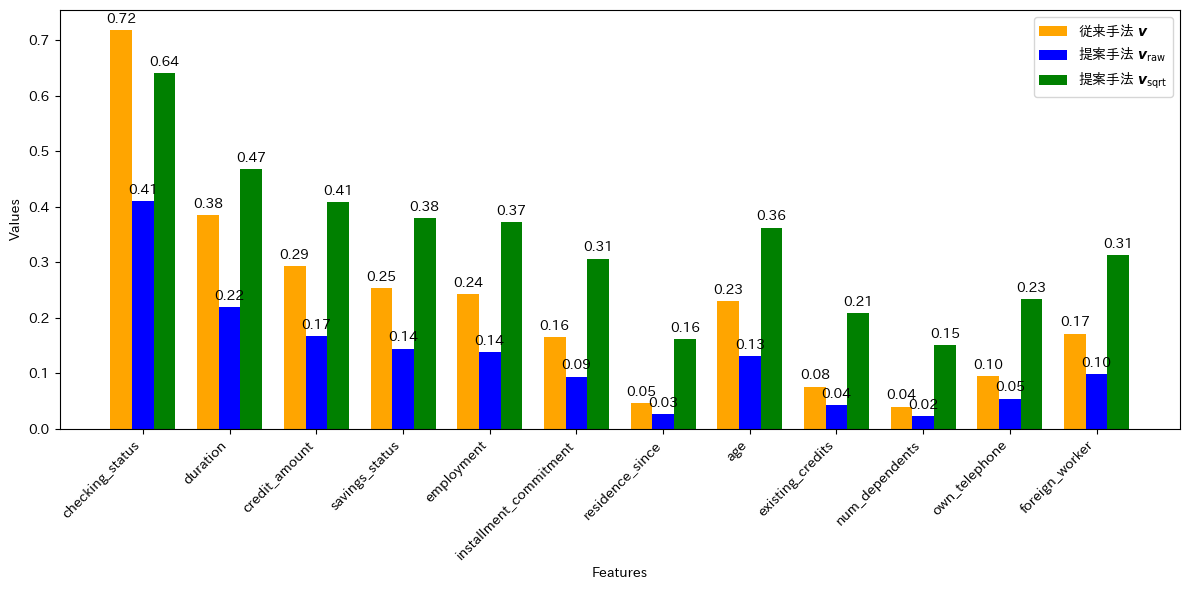
\includegraphics[width=0.8\textwidth]{images/実験_重要度算出の結果.png}
    \caption{実験結果:各特徴量における重要度}
    \label{fig:adversarial_example}
\end{figure}
重要度について比較すると,従来手法では,checking\_statusに対する重要度が飛び抜けており,次に重要度の高い特徴量との差が大きいことが指摘されていた.提案手法ではその差が小さくなっていることが確認できる.また,提案手法(式(8))では,特徴量の重要度がより均等になっていることがわかる.これにより,提案手法はより自然な敵対的サンプルを生成できることが示された.
\subsection{考察}
以上の実験結果を考察すると,提案手法は従来手法よりも元データに近い敵対的サンプルを生成することが示された.特に成功率および平均距離の指標では,提案手法(式(7))が従来手法を上回る性能を発揮した.この結果は,提案手法が重要度算出と離散化の適切な組み合わせにより,必要最小限のノイズで誤分類を誘発する敵対的サンプルを生成できたためと考えられる.一方で,重み距離の結果において提案手法(式(8))が劣る原因としては,重要度算出アルゴリズムにおける平方根操作の影響が挙げられる.平方根は大きい値を小さく小さい値を大きくするため図8で従来手法と比較するとより滑らかな重要度
となっている.分類性能に影響を与える重要な特徴量に対する変化が抑制されなかったことが考えられる.これにより自然な敵対的サンプルの生成を行うことができなかったということがわかる.

さらに,評価結果に基づき元データ,従来手法,提案手法(式(7))による敵対的サンプルを比較した結果,提案手法によるサンプルはより「自然」であり,実運用環境における敵対的サンプル対策として有効であることが確認された.

\begin{table}[H]
    \centering
    \caption{元データと敵対的サンプルの比較}
    \begin{tabular}{|c|c|c|c|} \hline
        特徴量 & 元データ & 従来手法 & 提案手法 \\ \hline
        checking\_status & 0 & 0.09115 & 0\\ \hline
        duration & 14 & 8.89098 & 15 \\ \hline
        credit\_amount & 8978 & 7153.84454 & 9169 \\ \hline
        savings\_status & 0 & 0.083762 & 0\\ \hline
        employment & 4 & 3.947638  & 4 \\ \hline
        installment\_commitment & 1 & 1.071917 & 1\\ \hline
        residence\_since & 4 & 4.000000 & 2 \\ \hline
        age & 45 & 44.413271 & 45 \\ \hline
        existing\_credits & 1 & 1.000000 & 1 \\ \hline
        num\_dependents & 1 & 1.000000 & 1 \\ \hline
        own\_telephone & 1 & 0.992310 & 1 \\ \hline
        foreign\_worker & 1 & 1.000000 & 1 \\ \hline
    \end{tabular}
\end{table}

実際のデータについても,離散化により自然な敵対的サンプルになっていることがわかる.また,ノイズの大きさについてもchecking\_statusのノイズを避けるあまり,durationやcredit\_amountに対してノイズが大きくなっている従来手法に対して,提案手法は小さくすることができている.これにより,提案手法はより自然な敵対的サンプルを生成できることが示された.